\documentclass[tikz, border=8pt]{standalone}
\usepackage{tikz}
\usetikzlibrary{positioning, arrows.meta, fit, backgrounds, calc}
\usepackage{amsmath}

%% Mode 3: Natural Labeled Soundscape Training (primary JEPA training mode)
%%
%% LEFT  — Soundscape window through context encoder → classification + slots
%% RIGHT — Species clips (fetched by soundscape labels) through target encoder
%%         → compose in LATENT SPACE → JEPA factor & composition targets
%%
%% The composition happens entirely in latent space — no audio mixing.

\definecolor{cIn} {RGB}{186,230,253}
\definecolor{cEc} {RGB}{ 30, 64,175}
\definecolor{cEt} {RGB}{ 71, 85, 99}
\definecolor{cP1} {RGB}{194, 65, 12}
\definecolor{cP2} {RGB}{109, 40,217}
\definecolor{cCl} {RGB}{ 22,101, 52}
\definecolor{cSl} {RGB}{254,215,170}
\definecolor{cLo} {RGB}{185, 28, 28}
\definecolor{cPL} {RGB}{229,240,253}
\definecolor{cPR} {RGB}{240,242,229}

\begin{document}
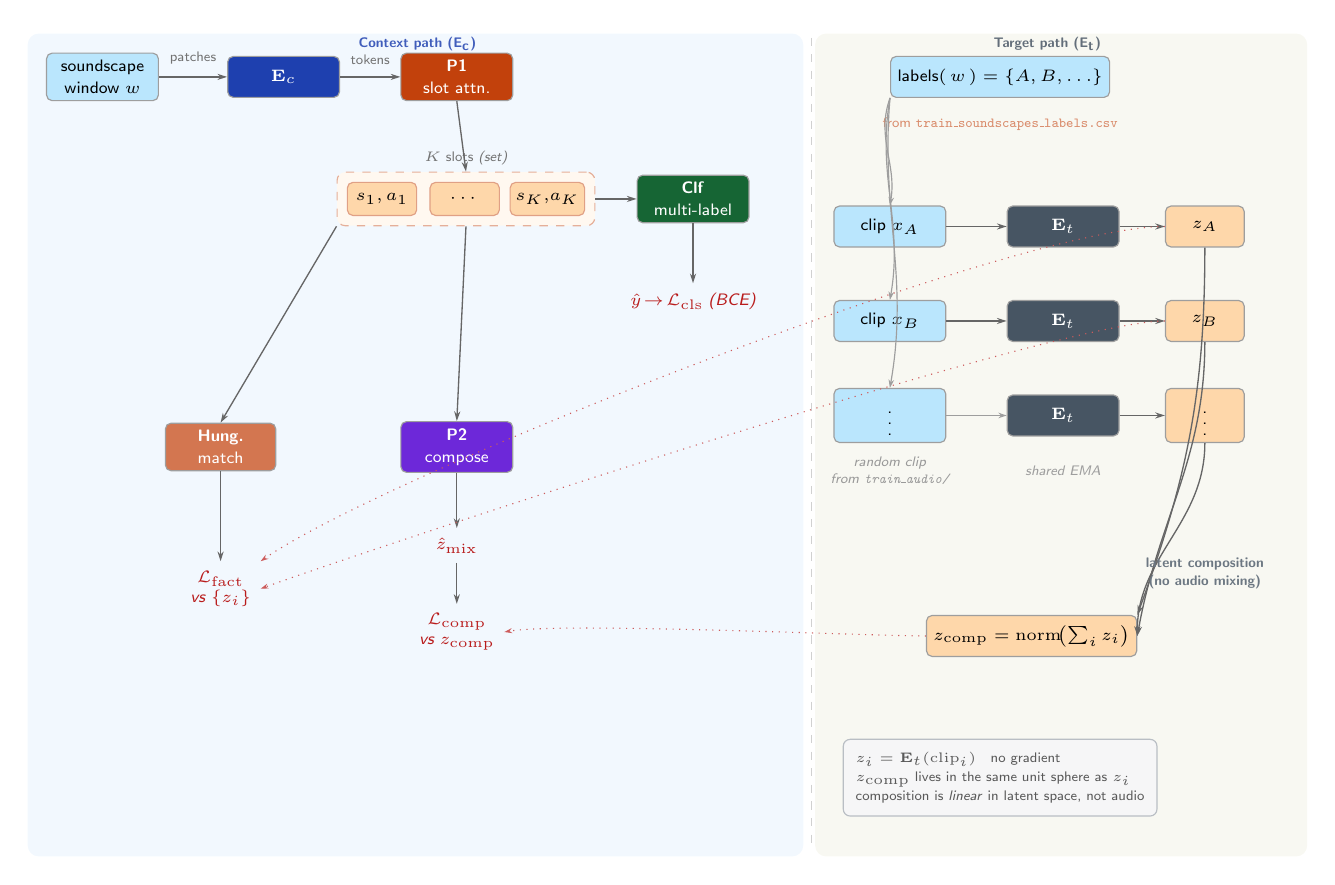
\begin{tikzpicture}[
  blk/.style={
    rectangle, rounded corners=2pt,
    draw=black!38, line width=0.42pt,
    align=center, minimum height=0.52cm, minimum width=1.42cm,
    inner sep=2.5pt, font=\fontsize{6.5}{8}\selectfont\sffamily
  },
  slt/.style={
    rectangle, rounded corners=2pt,
    draw=cP1!50, line width=0.42pt, fill=cSl,
    minimum height=0.42cm, minimum width=0.88cm,
    inner sep=2pt, font=\fontsize{6}{7}\selectfont\sffamily, align=center
  },
  fw/.style={
    -{Stealth[length=3.5pt,width=2.2pt]}, line width=0.48pt, black!60
  },
  fwg/.style={
    -{Stealth[length=3pt,width=2pt]}, line width=0.42pt, black!38
  },
  lcon/.style={
    -{Stealth[length=2.8pt,width=1.8pt]}, line width=0.4pt, dotted, cLo!72
  },
  ann/.style={
    font=\fontsize{5.5}{6.5}\selectfont\sffamily, text=black!55, align=center
  },
  loss/.style={
    font=\fontsize{6}{7.2}\selectfont\itshape\sffamily, text=cLo, align=center
  },
  hdr/.style={
    font=\fontsize{5.5}{6.5}\selectfont\bfseries\sffamily, align=center
  },
]

%% ── Background panels ────────────────────────────────────────────────────────
\begin{scope}[on background layer]
  \fill[cPL!50, rounded corners=4pt] (-0.95, 0.55) rectangle ( 8.90,-9.90);
  \fill[cPR!50, rounded corners=4pt] ( 9.05, 0.55) rectangle (15.30,-9.90);
\end{scope}

%% ────────────────────────────────────────────────────────────────────────────
%% LEFT PANEL — Context path: real soundscape through E_c → P1 → Clf
%% ────────────────────────────────────────────────────────────────────────────
\node[blk, fill=cIn] (sc) at (0.0, 0.0)
  {soundscape\\window $w$};
\node[blk, fill=cEc, text=white] (ec)  at (2.3, 0.0) {$\mathbf{E}_c$};
\node[blk, fill=cP1, text=white] (p1)  at (4.5, 0.0) {\textbf{P1}\\slot attn.};

\draw[fw] (sc) -- (ec) node[midway, above=1pt, ann] {patches};
\draw[fw] (ec) -- (p1) node[midway, above=1pt, ann] {tokens};

%% Slot box
\node[slt] (s1)   at (3.55, -1.55) {$s_1,a_1$};
\node[slt] (sdot) at (4.60, -1.55) {$\cdots$};
\node[slt] (sk)   at (5.65, -1.55) {$s_K,\!a_K$};

\begin{scope}[on background layer]
  \node[
    draw=cP1!42, line width=0.42pt, dashed, rounded corners=3pt,
    fill=cSl!18, inner sep=3.5pt,
    fit=(s1)(sk),
    label={[ann, yshift=-1pt]above:$K$ slots \textit{(set)}}
  ] (slotbox) {};
\end{scope}
\draw[fw] (p1.south) -- (slotbox.north);

%% Classifier (primary supervised loss)
\node[blk, fill=cCl, text=white] (clf) at (7.5, -1.55) {\textbf{Clf}\\multi-label};
\draw[fw] (slotbox.east) -- (clf.west);
\node[loss] (lcls) at (7.5, -2.85)
  {$\hat{y} \!\to\! \mathcal{L}_{\mathrm{cls}}$\;(BCE)};
\draw[fw] (clf) -- (lcls);

%% P2 compose (auxiliary JEPA path)
\node[blk, fill=cP2, text=white] (p2) at (4.5, -4.70) {\textbf{P2}\\compose};
\draw[fw] (slotbox.south) -- (p2.north);

\node[loss] (zhat)  at (4.5, -5.95) {$\hat{z}_{\mathrm{mix}}$};
\node[loss] (lcomp) at (4.5, -7.05)
  {$\mathcal{L}_{\mathrm{comp}}$\\vs $z_{\mathrm{comp}}$};
\draw[fw] (p2) -- (zhat);
\draw[fw] (zhat) -- (lcomp);

%% Hungarian match
\node[blk, fill=cP1!72, text=white, minimum width=1.4cm]
  (hung) at (1.5, -4.70) {\textbf{Hung.}\\match};
\draw[fw] (slotbox.south west) -- (hung.north);

\node[loss] (lfact) at (1.5, -6.50)
  {$\mathcal{L}_{\mathrm{fact}}$\\vs $\{z_i\}$};
\draw[fw] (hung) -- (lfact);

\node[hdr, text=cEc!85] at (4.0, 0.42) {Context path (E\textsubscript{c})};

%% ────────────────────────────────────────────────────────────────────────────
%% VERTICAL SEPARATOR
%% ────────────────────────────────────────────────────────────────────────────
\draw[black!18, dashed, line width=0.45pt] (9.0, 0.50) -- (9.0,-9.80);

%% ────────────────────────────────────────────────────────────────────────────
%% RIGHT PANEL — Target path: species clips → E_t → latent composition
%%               clips are selected from train_audio/ using soundscape labels
%% ────────────────────────────────────────────────────────────────────────────

%% Soundscape label box (shared knowledge from labels)
\node[blk, fill=cIn, minimum width=2.4cm] (lbl) at (11.4, 0.0)
  {labels$(\,w\,)=\{A,B,\ldots\}$};

\node[ann, text=cP1!60, font=\fontsize{5}{6}\selectfont\sffamily]
  at (11.4, -0.60)
  {from \texttt{train\_soundscapes\_labels.csv}};

%% Sample clips from train_audio/
\node[blk, fill=cIn] (xa)  at (10.0, -1.90) {clip $x_A$};
\node[blk, fill=cIn] (xb)  at (10.0, -3.10) {clip $x_B$};
\node[blk, fill=cIn] (xdot)at (10.0, -4.30) {$\vdots$};

\draw[fwg] (lbl.south west) to[out=250, in=80]  (xa.north);
\draw[fwg] (lbl.south west) to[out=260, in=80]  (xb.north);
\draw[fwg] (lbl.south west) to[out=265, in=80]  (xdot.north);

\node[ann, text=black!40, font=\fontsize{5}{6}\selectfont\itshape\sffamily]
  at (10.0,-5.00) {random clip\\from \texttt{train\_audio/}};

%% E_t encodes each clip
\node[blk, fill=cEt, text=white] (eta) at (12.2, -1.90) {$\mathbf{E}_t$};
\node[blk, fill=cEt, text=white] (etb) at (12.2, -3.10) {$\mathbf{E}_t$};
\node[blk, fill=cEt, text=white] (etd) at (12.2, -4.30) {$\mathbf{E}_t$};

\node[ann, text=black!38, font=\fontsize{5}{6}\selectfont\itshape\sffamily]
  at (12.2, -5.00) {shared EMA};

\draw[fw] (xa)   -- (eta);
\draw[fw] (xb)   -- (etb);
\draw[fwg](xdot) -- (etd);

%% Latent vectors
\node[blk, fill=cSl, minimum width=1.0cm] (za)  at (14.0, -1.90) {$z_A$};
\node[blk, fill=cSl, minimum width=1.0cm] (zb)  at (14.0, -3.10) {$z_B$};
\node[blk, fill=cSl, minimum width=1.0cm] (zdot)at (14.0, -4.30) {$\vdots$};

\draw[fw] (eta) -- (za);
\draw[fw] (etb) -- (zb);
\draw[fw] (etd) -- (zdot);

%% z_comp — composition in LATENT SPACE
\node[blk, fill=cSl, minimum width=2.3cm] (zcp) at (11.8, -7.10)
  {$z_{\mathrm{comp}} = \mathrm{norm}\!\bigl(\textstyle\sum_i z_i\bigr)$};

\draw[fw] (za.south)   to[out=270, in=70]  (zcp.north east);
\draw[fw] (zb.south)   to[out=270, in=80]  (zcp.east);
\draw[fw] (zdot.south) to[out=270, in=90]  (zcp.east);

\node[ann, text=cEt!80, font=\fontsize{5.5}{6.5}\selectfont\bfseries\sffamily]
  at (14.0, -6.30) {latent composition\\(no audio mixing)};

\node[hdr, text=cEt!85] at (12.0, 0.42) {Target path (E\textsubscript{t})};

%% ── Cross-path loss connections ───────────────────────────────────────────────
%% latents {z_i} → L_factored (Hungarian)
\draw[lcon] (za.west)  to[out=180, in=35, looseness=0.4] (lfact.north east);
\draw[lcon] (zb.west)  to[out=180, in=20, looseness=0.3] (lfact.east);
%% z_comp → L_comp
\draw[lcon] (zcp.west) to[out=180, in=10, looseness=0.35] (lcomp.east);

%% ────────────────────────────────────────────────────────────────────────────
%% LATENT SPACE NOTE
%% ────────────────────────────────────────────────────────────────────────────
\node[
  rectangle, rounded corners=2.5pt,
  draw=cEt!38, line width=0.42pt, fill=cEt!5,
  inner sep=4.5pt,
  font=\fontsize{5.5}{7}\selectfont\sffamily, align=left, text=black!65
] at (11.4, -8.90)
{
  $z_i = \mathbf{E}_t(\mathrm{clip}_i)$\quad no gradient\\
  $z_{\mathrm{comp}}$ lives in the same unit sphere as $z_i$\\
  composition is \textit{linear} in latent space, not audio
};

\end{tikzpicture}
\end{document}
